\documentclass[10pt,a4paper]{jarticle} %参考文献改ページ防ぐためにjarticleにしてるよ
\usepackage[top=20truemm,bottom=20truemm,left=20truemm,right=20truemm]{geometry}
\usepackage[dvipdfmx]{graphicx}
\usepackage{here}
\usepackage{amsmath}
\usepackage{url}
\usepackage{cases}
\usepackage{braket}
\usepackage{caption} %図表キャプションまわり
\captionsetup[figure]{format=plain, labelformat=simple, labelsep=space, font=footnotesize}
\captionsetup[table]{format=plain, labelformat=simple, labelsep=space, font=small}
%\renewcommand{\bibname}{} %jreportではデフォルトで関連図書とかになる

\begin{document}
\begin{center}
\bf{\LARGE ゼーベック係数$S$のキャリア濃度依存性について}
\end{center}
\begin{flushright}
N. H. Shimada
\end{flushright}

レポートで必要となり調べたが、ネット上にきちんとした数式での導出を行っている記述が見当たらなかったのでまとめたものを公開する。主に\cite{1}を参照している。ゼーベック効果は温度差$\Delta T$によって電位差$\Delta V$が生じる現象である。キャリアを正孔と仮定すれば、エネルギー準位は次の図のようになる。
\begin{figure}[ht]
\centering  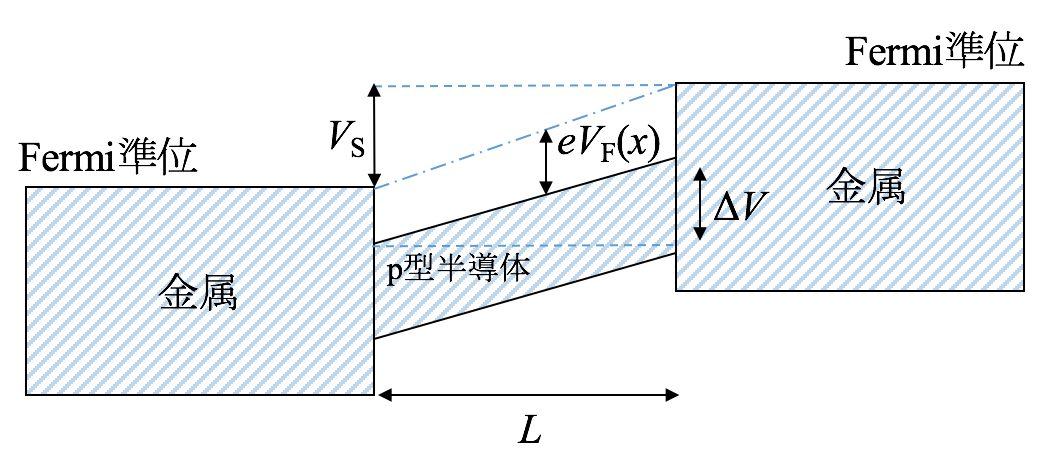
\includegraphics[width=10cm]{Fermi.png} 
\caption{エネルギー準位図。斜線部は価電子帯を表す。}
\label{Fermi}
\end{figure}\\
正孔分布の偏りによって電位差$\Delta V$が生じている。両端の金属板ではFermi準位が$V_S$違っており、これがゼーベック効果により生じた電位差である。$V_S$と$\Delta V$が等しくならないのは、Fermi準位が温度依存性を持ち、高温側と低温側でズレが生じるからである(高温ほど禁制帯の真ん中へと近づく、今の場合はよりエネルギーが高い方へとシフトする)。さて、温度勾配による拡散電流$I_{D}$と正孔分布による電位差から生じた電流$I_{E}$が釣り合っている時が定常状態であると考える。正孔濃度$p$として、
\begin{eqnarray}
I_D &=& eD_h \frac{dp}{dx} \\
&=& e \frac{kT\mu_F}{e}  \frac{dp}{dx} \\
I_E &=& ep\mu_F \Delta V \\
 &=& ep\mu_F \frac{\Delta V}{L}
\end{eqnarray}
係数$D_h$はアインシュタインの関係式から$D_h=\frac{kT\mu_F}{e}$を用いた。この2式が釣り合っているので、
\begin{eqnarray}
I_D &=& I_E \\
e \frac{kT\mu_F}{e}  \frac{dp}{dx} &=& ep\mu_F \frac{\Delta V}{L} \\
\frac{dp}{dx} &=& \frac{ep}{kT}  \frac{\Delta V}{L} 
\end{eqnarray}
ここで、
\begin{eqnarray}
\frac{dp}{dx} = \frac{dp}{dT} \frac{dT}{dx} = \frac{dp}{dT} \frac{\Delta T}{L}
\end{eqnarray}
を使うと次のようになる。
\begin{eqnarray}
\frac{dp}{dT} = p \frac{e}{kT} \frac{\Delta V}{\Delta T}
\end{eqnarray}
正孔濃度$p$の温度依存性は、$p = U_h T^{3/2} \mathrm{exp}(-\frac{eV_F(T)}{kT})$の式からわかっているとして、これを用いると、
\begin{eqnarray}
\Delta V = \Delta T \left( \frac{3}{2}\frac{k}{e} + \frac{V_F}{T} - \frac{dV_F}{dT} \right)
\end{eqnarray}
のように変形できる。電位差$V_S$は$\Delta V$との差を考慮すると、次のように書ける。
\begin{eqnarray}
V_S = \Delta V + \frac{dV_F}{dT}\Delta T
\end{eqnarray}
上二式より、
\begin{eqnarray}
V_S = \Delta T \left(\frac{3}{2}\frac{k}{e} + \frac{V_F}{T} \right)
\end{eqnarray}
よってゼーベック係数は、
\begin{eqnarray}
S &=& \frac{3}{2}\frac{k}{e} + \frac{V_F}{T}  \\
&=& \frac{3}{2}\frac{k}{e} - \frac{k}{e} \, \mathrm{ln} \left( \frac{p}{U_h T^{\frac{3}{2}}} \right)
\end{eqnarray}
最終的に正孔濃度依存性を見るために、$p$を含む表式へ書き換えた。

\begin{thebibliography}{999}
\bibitem{1} 高橋清/山田陽一 「半導体工学 半導体物性の基礎」 p197-199 (森北出版株式会社)
\end{thebibliography}

\end{document}